\documentclass[rgb,dvipsnames,aspectratio=169]{beamer}
\usepackage[english]{babel}
\usepackage[utf8]{inputenc}
\usepackage{xcolor}
\usepackage{listings}
\usepackage{adjustbox}
\usepackage{amsmath}
\usepackage{multirow}
\usepackage{amsfonts}
\usepackage{url}
\usepackage[linewidth=1pt]{mdframed}
\usepackage{alltt}
\usepackage{graphicx}
\usepackage{tikz}
\usetikzlibrary{calc,shapes.multipart,chains,arrows,patterns}
\usepackage{paratype}
\setbeamerfont{frametitle}{family=\bf}
\usepackage{pgfplots}

\usecolortheme{seagull}
\usecolortheme{whale}
\setbeamertemplate{itemize item}{\raisebox{0.8mm}{\rule{1.2mm}{1.2mm}}}
\usenavigationsymbolstemplate{} % no navigation buttons

\newcommand{\sem}[1]{[\![\,#1\,]\!]}
\newcommand{\seme}[1]{\sem{#1}\varepsilon}
\newcommand{\semzero}[1]{\sem{#1}_0}

\newcommand{\emptymap}{\{\}}
\newcommand{\fracc}[2]{\begin{eqnarray} \frac{\begin{array}{c} #1
    \end{array}}{\begin{array}{c} #2 \end{array}} \end{eqnarray}}
\newcommand{\sembox}[1]{\hfill \normalfont \mbox{\fbox{\(#1\)}}}
\newcommand{\sempart}[2]{\subsubsection*{\rm\em #1 \sembox{#2}}}
\newcommand{\axiom}[1]{\begin{eqnarray} \begin{array}{c} #1 \end{array} \end{eqnarray}}
\newcommand{\fraccn}[2]{\refstepcounter{equation}\mbox{$\frac{\begin{array}{c} #1 \end{array}}{\begin{array}{c} #2 \end{array}}$}~(\arabic{equation})}
\newcommand{\fraccc}[2]{\mbox{$\frac{\begin{array}{c} #1 \end{array}}{\begin{array}{c} #2 \end{array}}$}}
\newcommand{\onepart}[1]{\noindent\hfill#1\hfill~\vspace{2mm}}
\newcommand{\twopart}[2]{\noindent\hfill#1\hfill#2\hfill~\vspace{2mm}}
\newcommand{\threepart}[3]{\noindent\hfill#1\hfill#2\hfill#3\hfill~\vspace{2mm}}
%\newcommand{\axiomm}[1]{\refstepcounter{equation}\mbox{$\begin{array}{c} #1 \end{array}$}~(\arabic{equation})}
\newcommand{\axiomm}[1]{$\begin{array}{c} #1 \end{array}$}
%\newcommand{\ar}[1]{\stackrel{#1}{\longrightarrow}}
\newcommand{\vd}{\vdash}
\newcommand{\Ran}{{\rm Ran}}
\newcommand{\Dom}{{\rm Dom}}
%\newcommand{\kw}[1]{\texttt{#1}}
\newcommand{\id}[1]{\mbox{\it{#1}}}
\newcommand{\rarr}{\rightarrow}
\newcommand{\eval}{\rarr}
\newcommand{\evals}{\leadsto}
\newcommand{\larr}{\leftarrow}

% Beamer theme settings

\definecolor{black}{RGB}{0,0,0}
\definecolor{maroon}{RGB}{128,0,0}
\definecolor{olive}{RGB}{128,128,0}
\definecolor{green}{RGB}{0,128,0}
\definecolor{purple}{RGB}{128,0,128}
\definecolor{teal}{RGB}{0,128,128}
\definecolor{darkteal}{RGB}{0,92,92}
\definecolor{navy}{RGB}{0,0,128}
\definecolor{gray}{RGB}{128,128,128}
\definecolor{darkgray}{RGB}{60,60,60}
\definecolor{darkred}{RGB}{139,0,0}

%palette

% #173F5F (dark blue)
\definecolor{darkblue}{RGB}{23,63,95}
% #20639B (blue)
\definecolor{blue}{RGB}{32,99,155}
% #3CAEA3 (green)
\definecolor{magenta}{RGB}{60,174,163}
% #F6D55C (yellow)
\definecolor{yellow}{RGB}{246,213,92}
% #ED553B (red)
\definecolor{red}{RGB}{237,85,59}

\newcommand{\setallthemecolors}[1]{%
\setbeamercolor*{palette primary}{use=structure,fg=white,bg=#1}%
\setbeamercolor*{palette secondary}{use=structure,fg=white,bg=#1}%
\setbeamercolor*{palette tertiary}{use=structure,fg=white,bg=#1}}

\definecolor{mydarkred}{rgb}{.7,0,0}
\definecolor{mydarkblue}{rgb}{0,0,.7}
\definecolor{mydarkgreen}{rgb}{0,.7,0}
\definecolor{KUred}{RGB}{114, 0, 18}  % Gray  Approximate PANTONE COOL-GRAY-8
\newcommand{\Red}[1]{\textcolor{mydarkred}{#1}}
\newcommand{\Blue}[1]{\textcolor{mydarkblue}{#1}}
%\newcommand{\ar}[1]{\stackrel{#1}{\longrightarrow}}
\newcommand{\ar}[1]{\mathop{\vbox{\ialign{##\crcr % right arrow with
                                                  % argument on top
       \noalign{\kern 2pt\nointerlineskip}\crcr
       $\hfil\scriptstyle\kern 6pt{#1}\kern 6pt\hfil$\crcr
       \noalign{\kern-0pt\nointerlineskip}\crcr
       \rightarrowfill\crcr}}}\nolimits}

\newcommand{\putat}[3]{\begin{picture}(0,0)(0,0)\put(#1,#2){#3}\end{picture}}

\newcommand{\hl}[1]{\textbf{\emph{#1}}}

\newcommand{\Sep}{\hspace{2mm}|\hspace{2mm}}
\newcommand{\kw}[1]{\ensuremath{\mathtt{#1}}}
\newcommand{\ket}[1]{| #1 \rangle}
\newcommand{\twovec}[2]{\begin{bmatrix}#1 \\ #2\end{bmatrix}}
\newcommand{\hadamard}{\frac{1}{\sqrt{2}}\twovec{1 & 1}{1 & -1}}
\newcommand{\vect}[1]{\begin{bmatrix}#1\end{bmatrix}^{\rm T}}
%\newcommand{\sem}[1]{[\![#1]\!]}
\newcommand{\semd}[1]{\mathcal{I}[#1]}
\newcommand{\C}{\mathbb{C}}
\newcommand{\N}{\mathbb{N}}
\newcommand{\rar}{\rightarrow}
%\newcommand{\id}[1]{\ensuremath{\mathit{#1}}}
\newcommand{\T}{T}
\newcommand{\rbox}[1]{{\setlength{\fboxsep}{2pt}\color{KUred}{\fbox{\color{black}{#1}}}}}
\newcommand{\crbox}[1]{{\setlength{\fboxsep}{0pt}\color{KUred}{\fbox{\color{black}{#1}}}}}
\newcommand{\Let}{\mathtt{let}}
\newcommand{\Def}{\mathtt{def}}
\newcommand{\In}{\mathtt{in}}
\renewcommand{\eqref}[1]{\stackrel{\ref{#1}}{=}}
\newcommand{\eqreff}[2]{\stackrel{\ref{#1},\ref{#2}}{=}}
\newcommand{\dq}{{\color{mydarkblue}{dq}}}

\newcommand{\head}[1]{\vspace{3mm} \textbf{\normalsize #1}}
\newcommand{\size}{\ensuremath{\mathrm{size}}}
\renewcommand{\log}{\ensuremath{\mathrm{log}}}
\renewcommand{\sp}{\vspace{1ex}}
\newcommand{\shead}[1]{\vspace{1ex}\head{#1}\vspace{1ex}}

\newcommand{\fblock}[2]{\framebox[#1][t]{~\hfill\begin{tabular}{c}#2\end{tabular}\hfill~}}

\setallthemecolors{navy}

\useoutertheme{infolines}
\useinnertheme{rectangles}

\title{PLTC BSc Projects 2025}

\author[Martin Elsman]{Martin Elsman}
\institute[PLTC]{PLTC Section, DIKU}

\date[June 27, 2025]{{June 27, 2025}\makebox(0,0){\vspace{0cm}\hspace{7cm}\begin{tabular}{c}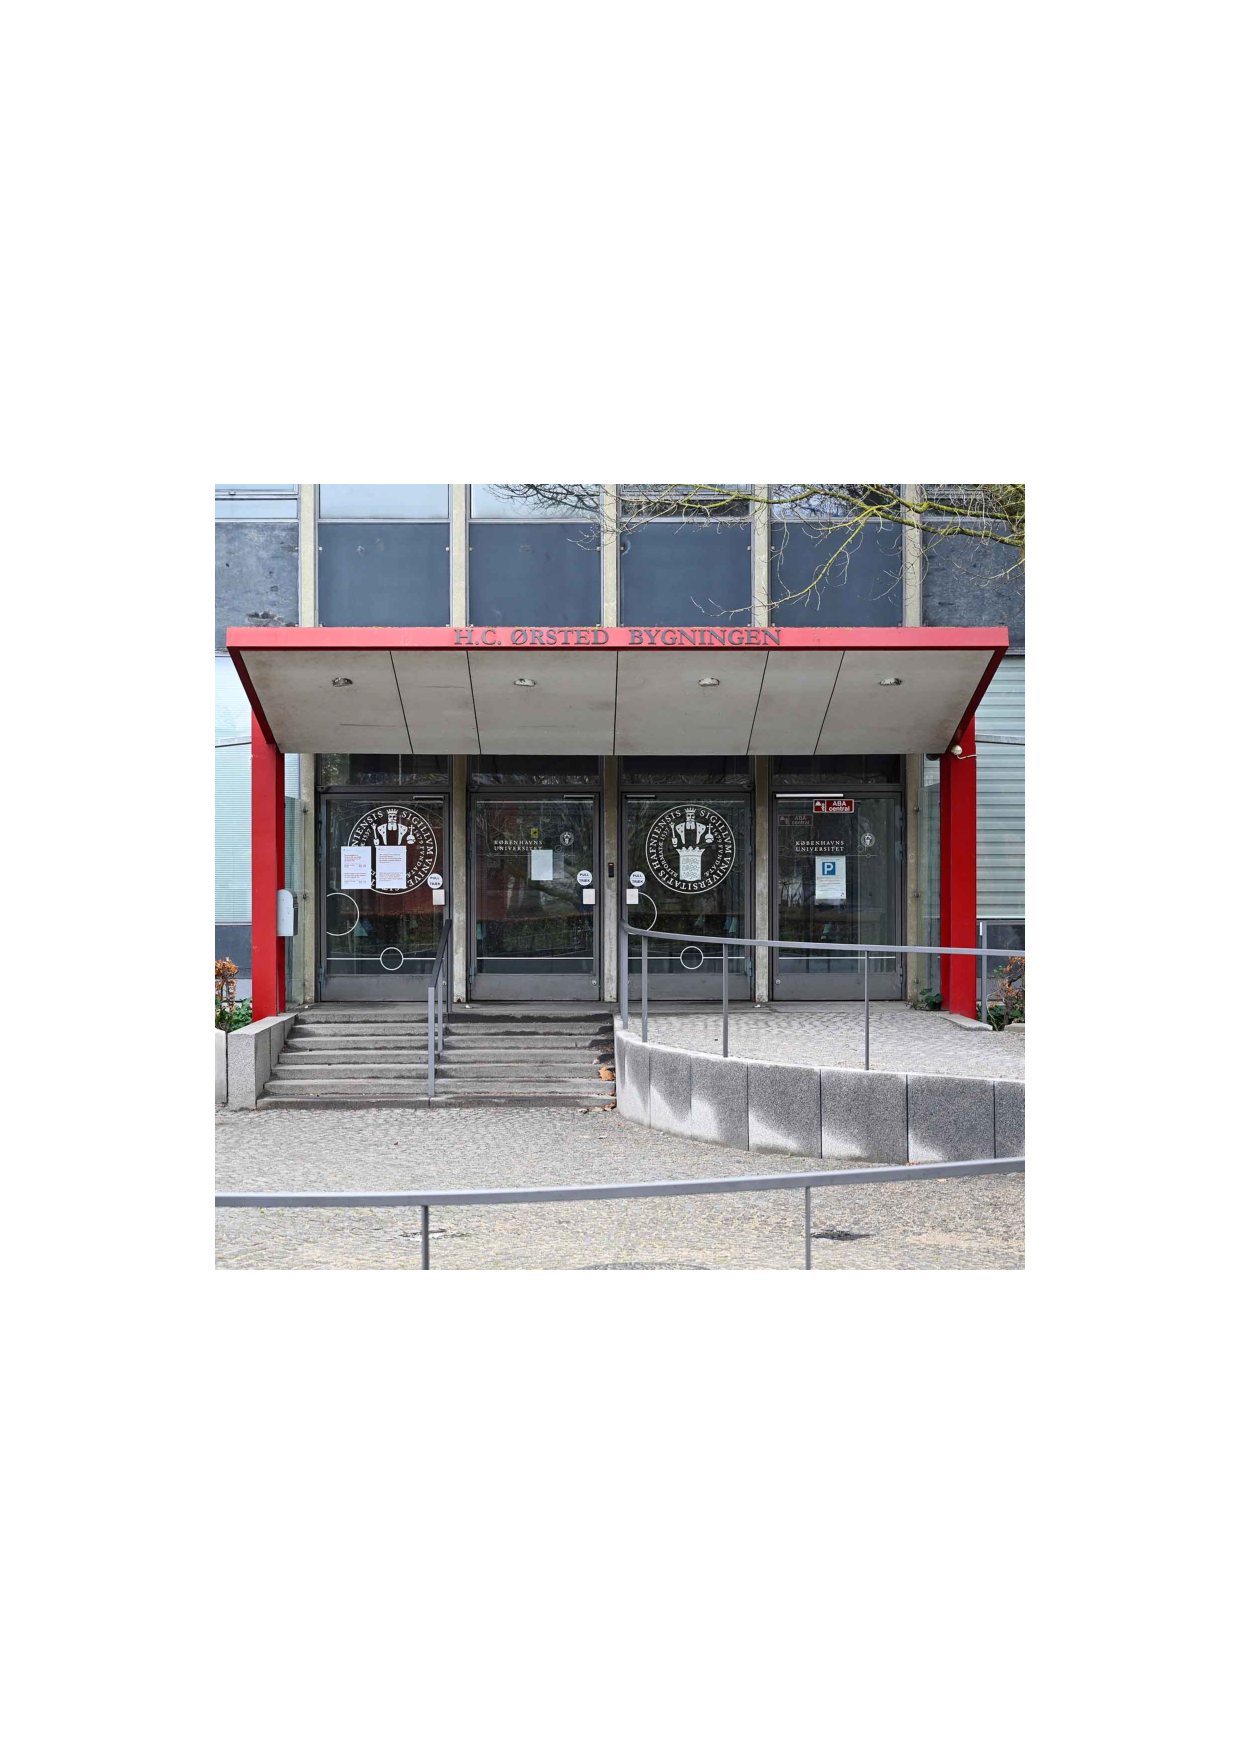
\includegraphics[width=6cm]{hco}\end{tabular}}
  \makebox(0,0){\vspace{0.5cm}\hspace{-12.5cm}\large BSc Project Event}
  \makebox(0,0){\vspace{-0.5cm}\hspace{-12.5cm}\large Fall 2025}
}

\setbeamertemplate{headline}{}
\begin{document}

\frame{\titlepage}

\begin{frame}[fragile]
\head{The PLTC Section}

\vfill

\begin{itemize}
\item We perform research in programming language technology and in the theory of computation.

\vfill

\item Much of our work involves topics in the intersection of

\vfill
\begin{center}

\textbf{\large programming language theory}

(e.g., type systems, compilers, and formal verification)

\vfill

and

\vfill

\textbf{\large applications}

(e.g., security and privacy, systems,
distributed ledgers, fintech, quantum)
\end{center}
\end{itemize}

\end{frame}

\begin{frame}[fragile]

  \head{Programming Languages Are Tools But They Are Also Research Objects!}

  \vfill

\begin{verbatim}
How should we implement and design good programming languages?
What does "good" mean?

What does correctness mean?

What does it take for software to be secure?

How can we organize parallel computations optimally?

What does "optimal" mean?

(...)
\end{verbatim}

\end{frame}

\begin{frame}[fragile]

  \head{Research Interests (I)}

  \vfill

  \begin{itemize}
  \item Compilation and optimisation.
    \emph{(Torben Mogensen, Cosmin Oancea, Martin Elsman, Troels Henriksen, Andrzej Filinski).}

    Related courses: PMPH, PLD, IPS.

  \item Logic and Semantics.
    \emph{(Andrzej Filinski, Robert Glück, …).}

    Related courses: LiCS, SaT.

  \item Type systems and type inference.
    \emph{(Andrzej Filinski, Troels Henriksen, Martin Elsman, Robert Glück, Torben Mogensen).}

    Related courses: SaT.

  \item Data-parallel and GPU programming.
    \emph{(Cosmin Oancea, Troels Henriksen, Martin Elsman).}

    Related courses: PMPH, DPP.

  \item Reversible languages and quantum computing.
    \emph{(Robert Glück, Torben Mogensen, Michael Kirkedal Thomsen, Fritz Henglein, Martin Elsman).}

    Related courses: PAT, ATPL.

  \end{itemize}
\end{frame}

\begin{frame}[fragile]

  \head{Research Interests (II)}

  \vfill

  \begin{itemize}

  \item High-performance computing.
    \emph{(Cosmin Oancea, James Avery, David Marchant).}

    Related courses: PMPH, COMPSYS, HPPS.

  \item Probabilistic programming.
    \emph{(Thomas Hamelryck).}

    Related courses: …

  \item Security and language-based security.
    \emph{(Boel Nelson, Thomas Jensen, Andrzej Filinski).}

    Related courses: ITS, SOS, PCS.

  \item Systems and hardware-near programming.
    \emph{(Philippe Bonnet).}

    Related courses: COMPSYS, HPPS, ACS, DIS.

  \item Finance, contracts, and distributed systems.
    \emph{(Omry Ross, Fritz Henglein).}

    Related courses: DATFIN, Blockchain.
  \end{itemize}

\end{frame}

\begin{frame}[fragile]

  \head{More Information}

  \vfill
  \begin{itemize}
  \item \textbf{PLTC Web Pages:}

    \url{https://di.ku.dk/english/research/pltc/} (official)

    \url{https://diku-dk.github.io/pltc/} (internal)

    \vfill

  \item \textbf{PLTC Researchers:}

    \url{https://di.ku.dk/english/staff/vip/researchers_pltc/}

  \end{itemize}

\end{frame}
\end{document}
